\item \textbf{Try modeling the residuals as an AR process. Use the tools at your disposal to decide on an appropriate order and analyse the results. What is the impact of selecting different orders on the remaining residuals?}





%so these are my starting points
%must be stationary
%these two plot do not tell us much
\textit{For this part, we need to select the order of the \gls{AR} term (p). Therefore, \gls{PACF} and \gls{ACF} were plotted at the first step (see figures \ref{fig:Ass1_D1_PACF_ACF_X} and \ref{fig:Ass1_D2_PACF_ACF_X}).}  

\begin{figure}[H]
    \centering
    \begin{minipage}[b]{1\textwidth}
        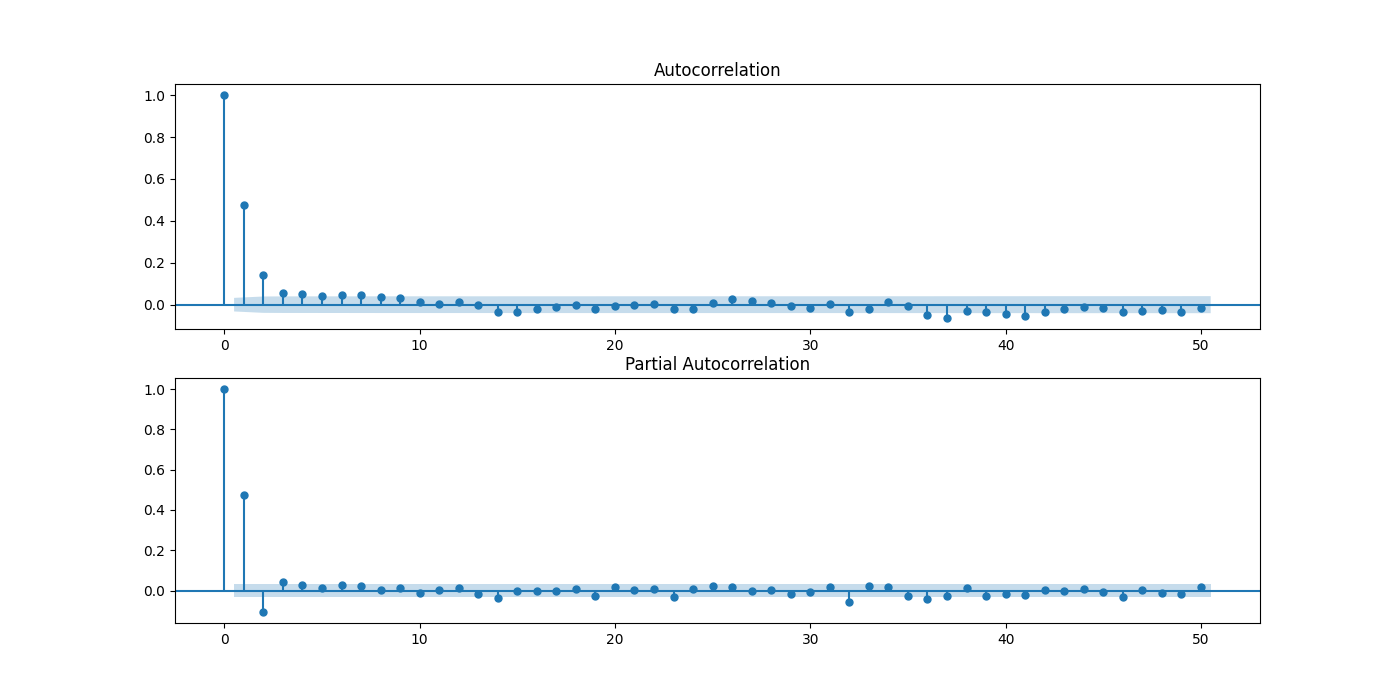
\includegraphics[width=\textwidth]{figures/Ass1/Ass1_D1_PACF_ACF_X.png}
    \end{minipage}
    \caption{A plot of the \gls{PACF} and \gls{ACF} on the residual part of the first dataset (residual of the STL method).}
    \label{fig:Ass1_D1_PACF_ACF_X}
\end{figure}

\begin{figure}[H]
    \centering
    \begin{minipage}[b]{1\textwidth}
        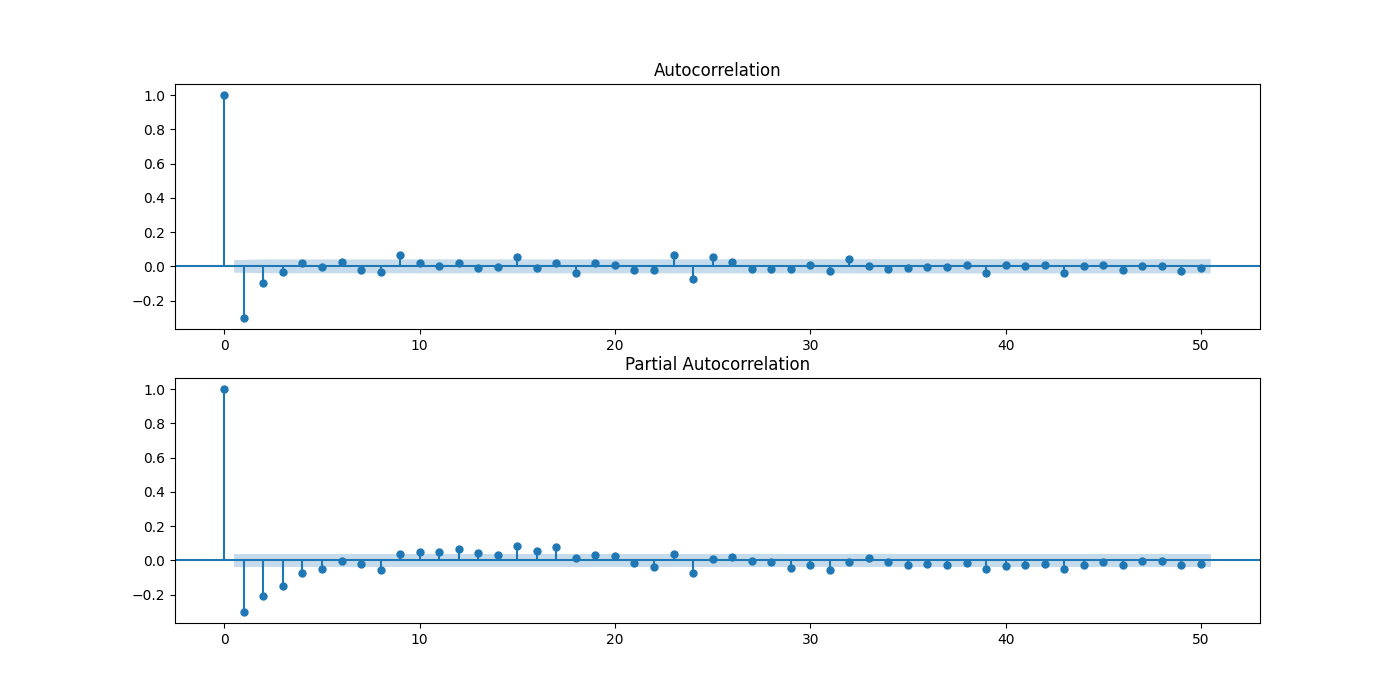
\includegraphics[width=\textwidth]{figures/Ass1/Ass1_D2_PACF_ACF_X.png}
    \end{minipage}
    \caption{A plot of the \gls{PACF} and \gls{ACF} on the residual part of the second dataset (residual of the STL method).}
    \label{fig:Ass1_D2_PACF_ACF_X}
\end{figure}


\textit{Since \gls{ACF} is decaying in both figures, it can conclude that these processes are an Auto-Regressive process. Also, based on \gls{PACF} in the first plot (figure \ref{fig:Ass1_D1_PACF_ACF_X}), the order of the \gls{AR} model should be either 1 and 2 due to these two lags have a significant value. Likewise, for the second dataset, we should select p a value between 1 to 4 (see figure \ref{fig:Ass1_D2_PACF_ACF_X}).}

\begin{figure}[H]
    \centering
    \begin{minipage}[b]{1\textwidth}
        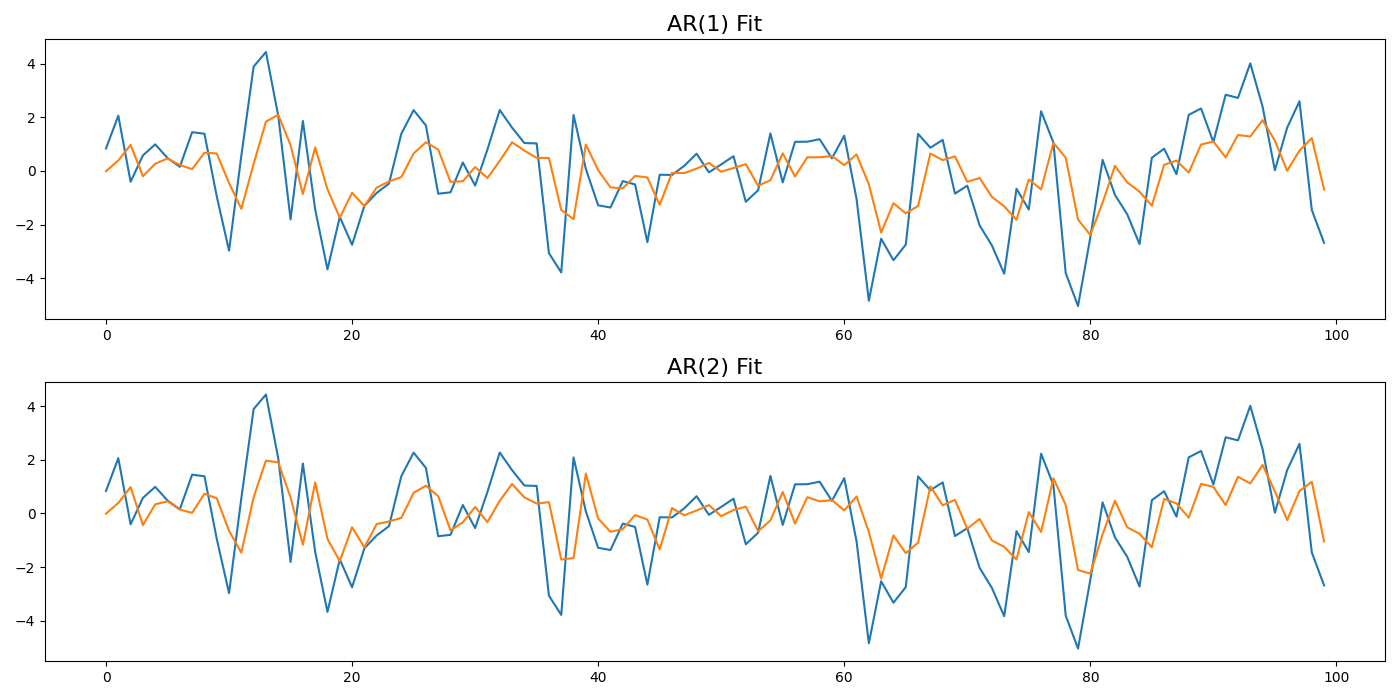
\includegraphics[width=\textwidth]{figures/Ass1/Ass1_D1_ARs models.png}
    \end{minipage}
    \caption{A part of residual signal (blue) and the fitted values (orange) for the first dataset.}
    \label{fig:Ass1_D1_ARs_models}
\end{figure}

\begin{figure}[H]
    \centering
    \begin{minipage}[b]{1\textwidth}
        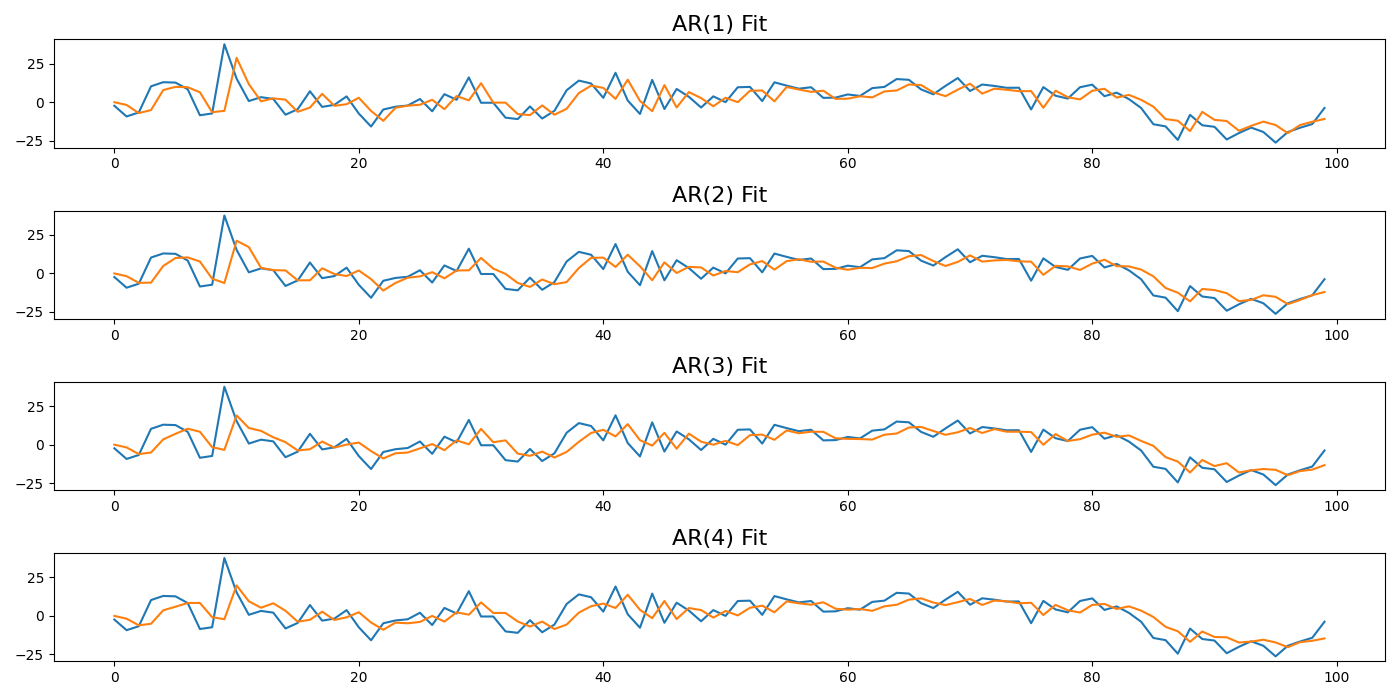
\includegraphics[width=\textwidth]{figures/Ass1/Ass1_D2_ARs models.png}
    \end{minipage}
    \caption{A part of residual signal (blue) and the fitted values (orange) for the second dataset.}
    \label{fig:Ass1_D2_ARs_models}
\end{figure}


\textit{Figures \ref{fig:Ass1_D1_ARs_models} and \ref{fig:Ass1_D2_ARs_models} indicate the output of our models on the datasets. As these two figures indicate, it is hard to select the best model based on the trained signal. Therefore, we need some criteria to help us to find the best model. Tables \ref{tab:Ass1_D1_AR} and \ref{tab:Ass1_D2_AR} show these criteria on these models. }

\begin{table}[H]
\centering
\caption{Comparing the \gls{AR} models in the first dataset.}
\label{tab:Ass1_D1_AR}
\begin{tabular}{lll}
\toprule
{} &  AR(1) &  AR(2) \\
\midrule
AR order  &      1 &      2 \\
AIC       &  1.288 &  1.277 \\
BIC       &  1.293 &  1.284 \\
RMS error &  1.149 &  1.156 \\
\bottomrule
\end{tabular}

\end{table}

\begin{table}[H]
\centering
\caption{Comparing the \gls{AR} models in the second dataset.}
\label{tab:Ass1_D2_AR}
\begin{tabular}{lllll}
\toprule
{} &      AR(1) &      AR(2) &      AR(3) &      AR(4) \\
\midrule
lag(s)      &          1 &          2 &          3 &          4 \\
AIC         &  22359.771 &  22236.837 &  22136.843 &  22097.596 \\
BIC         &  22377.589 &  22260.594 &  22166.538 &  22133.231 \\
RMS error   &      7.777 &      8.629 &     10.069 &     11.047 \\
Correlation &      0.522 &      0.457 &      0.401 &      0.335 \\
MPE         &     -0.618 &      0.046 &      0.739 &      1.149 \\
MAE         &      5.994 &      6.706 &      7.953 &      9.017 \\
\bottomrule
\end{tabular}

\end{table}

\textit{Figures \ref{fig:Ass1_D1_ARs_models} and \ref{fig:Ass1_D2_ARs_models} indicate the output of our models on the datasets.}


\textit{\Gls{AIC} and \gls{BIC} show the simplicity and goodness of an \gls{AR} model. If a model has a lower \Gls{AIC} and \gls{BIC}, it will be generally better than others. So for the first dataset, \gls{AR}(2) is better than \gls{AR}(1), and for the second dataset, \gls{AR}(4) is lower than among others.}

\textit{Figures \ref{fig:Ass1_D1_AR} and \ref{fig:Ass1_D2_AR} show the result of the model on testing set.} 

\begin{figure}[H]
    \centering
    \begin{minipage}[b]{1\textwidth}
        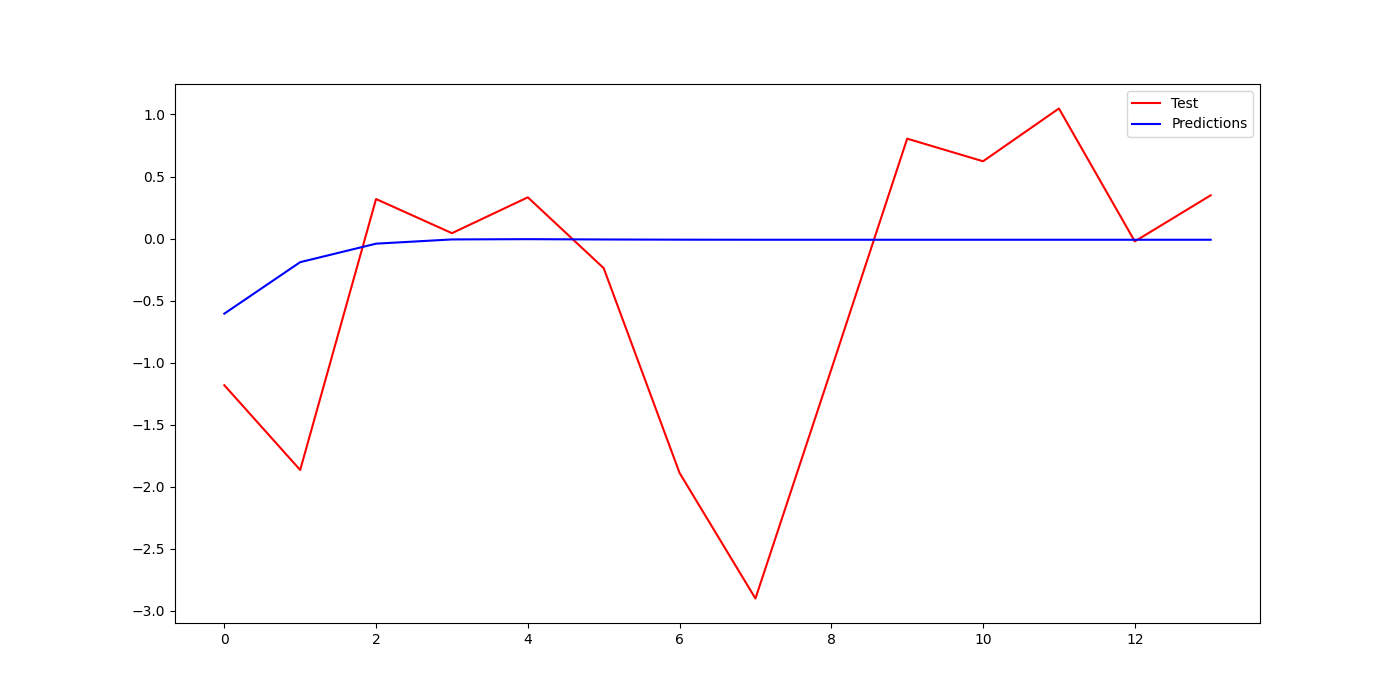
\includegraphics[width=\textwidth]{figures/Ass1/Ass1_D1_AR.png}
    \end{minipage}
    \caption{The prediction and holding out set (testing set) of the first dataset. }
    \label{fig:Ass1_D1_AR}
\end{figure}

\begin{figure}[H]
    \centering
    \begin{minipage}[b]{1\textwidth}
        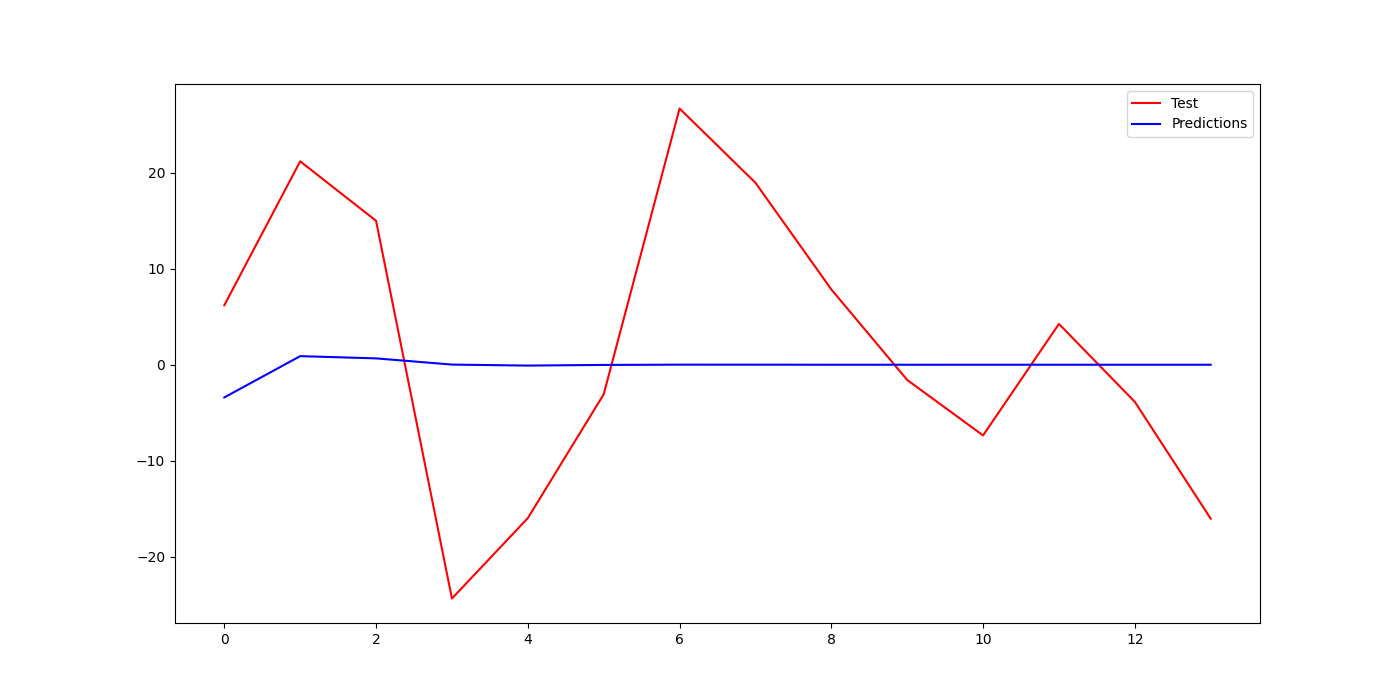
\includegraphics[width=\textwidth]{figures/Ass1/Ass1_D2_AR.png}
    \end{minipage}
    \caption{The prediction and holding out set (testing set) of the second dataset. }
    \label{fig:Ass1_D2_AR}
\end{figure}